\section{Beispiele}
\label{sec:Beispiele}


\subsection{Beispiel f�r die Erstellung von Formeln}
\label{sec:Beispielf�rdieErstellungvonFormeln}

Formeln werden eingef�gt unter: Einf�gen $\rightarrow$ Formeln  \\
Die jeweiligen Unterschiede bei den m�glichen Typen lassen sich durch "`ausprobieren"' erlernen! \\

BEISPIEL:

..... Dabei kommt es durch die reduzierten Widerstandsmomente zu einer Erh�hung und durch die Minderung der elastischen L�nge zu einer Reduktion der L�ngsspannungen in der Schiene. Dies wird aus der in Kapitel \ref{sec:Kapitel1} hergeleiteten Gleichung f�r die maximale Schienenl�ngsspannung infolge einer vertikalen Einzellast ersichtlich:  

	\begin{equation}
		\sigma_{xx}=\frac{Q(\xi)\cdot \sqrt[4]{\frac{4\cdot E_{E} \cdot I_{E}}{b_{E}\cdot k}} \cdot 0,25}{W_{y_{unten}}} = \frac{Q(\xi)\cdot \sqrt[4]{\frac{4\cdot E_{E}}{b_{E}\cdot k}}\cdot z_{u}}{4 \cdot I_{E}^{0,75}}
		\label{eq:spannung_elast}
	\end{equation} 
	
Auf �hnliche Weise l�sst sich auch eine Matrix darstellen:

BEISPIEL:
	
...F�r ein Scheibenelement ergibt sich beispielsweise folgender Ansatz f�r die Diskretisierung des Verschiebungsfeldes:

\begin{equation}
\begin{bmatrix} u \\ v	\end{bmatrix}_{(e)} = \begin{bmatrix} \phi^{T}_{u}(x,y) & 0 \\ 0 & \phi^{T}_{v}(x,y)	\end{bmatrix}_{(e)} \begin{bmatrix} U_u \\ U_v	\end{bmatrix}_{(e)}	
\end{equation}
	
	
	
\subsection{Zitate einf�gen}
\label{sec:ZitateEinf�gen}

Als erstes ist es erforderlich die vorhandene Literatur in dem Programm "`Jabref"' einzutragen! Dies ist auf einfache Weise m�glich.Das Benutzerhandbuch findet sich unter 
\href{http://jabref.sourceforge.net/manuals/JabRef-UserManual_de.pdf} {Benutzerhandbuch - Jabref}

Zitate werden folgenderma�en eingef�gt: \citep{Bathe2002} \\
Es ist i.d.R. erforderlich hierf�r 3 mal nacheinander zu kompilieren bzw. das Dokument zu erstellen!\\
(Das Erstellen l�sst sich �brigens auch mit der Tastenkombination "`Strg+F5"' durchf�hren)\\
Nachdem die Quelle aufgerufen wurde, wird der entsprechende Eintrag im Literaturverzeichnis automatisch erstellt!

\subsection{Bilder einf�gen}
\label{sec:BilderEinf�gen}

Um Bilder einzuf�gen einfach das entsprechende Bild in dem Ordner "`bilder"' ablegen und wie folgt beschrieben einf�gen. Um den wunderbaren Vorteil von LaTeX zu nutzen, dass Vektorgrafiken eingebunden werden k�nnen, bitte das Bild in dem Format "`pdf"' abspeichern und eingescannte Bilder entsprechend mit hoher Qualit�t erstellen!

Bilder lassen sich einf�gen unter: Einf�gen $\rightarrow$ Grafik

Beispiel:

\begin{figure}[H]
	\centering
		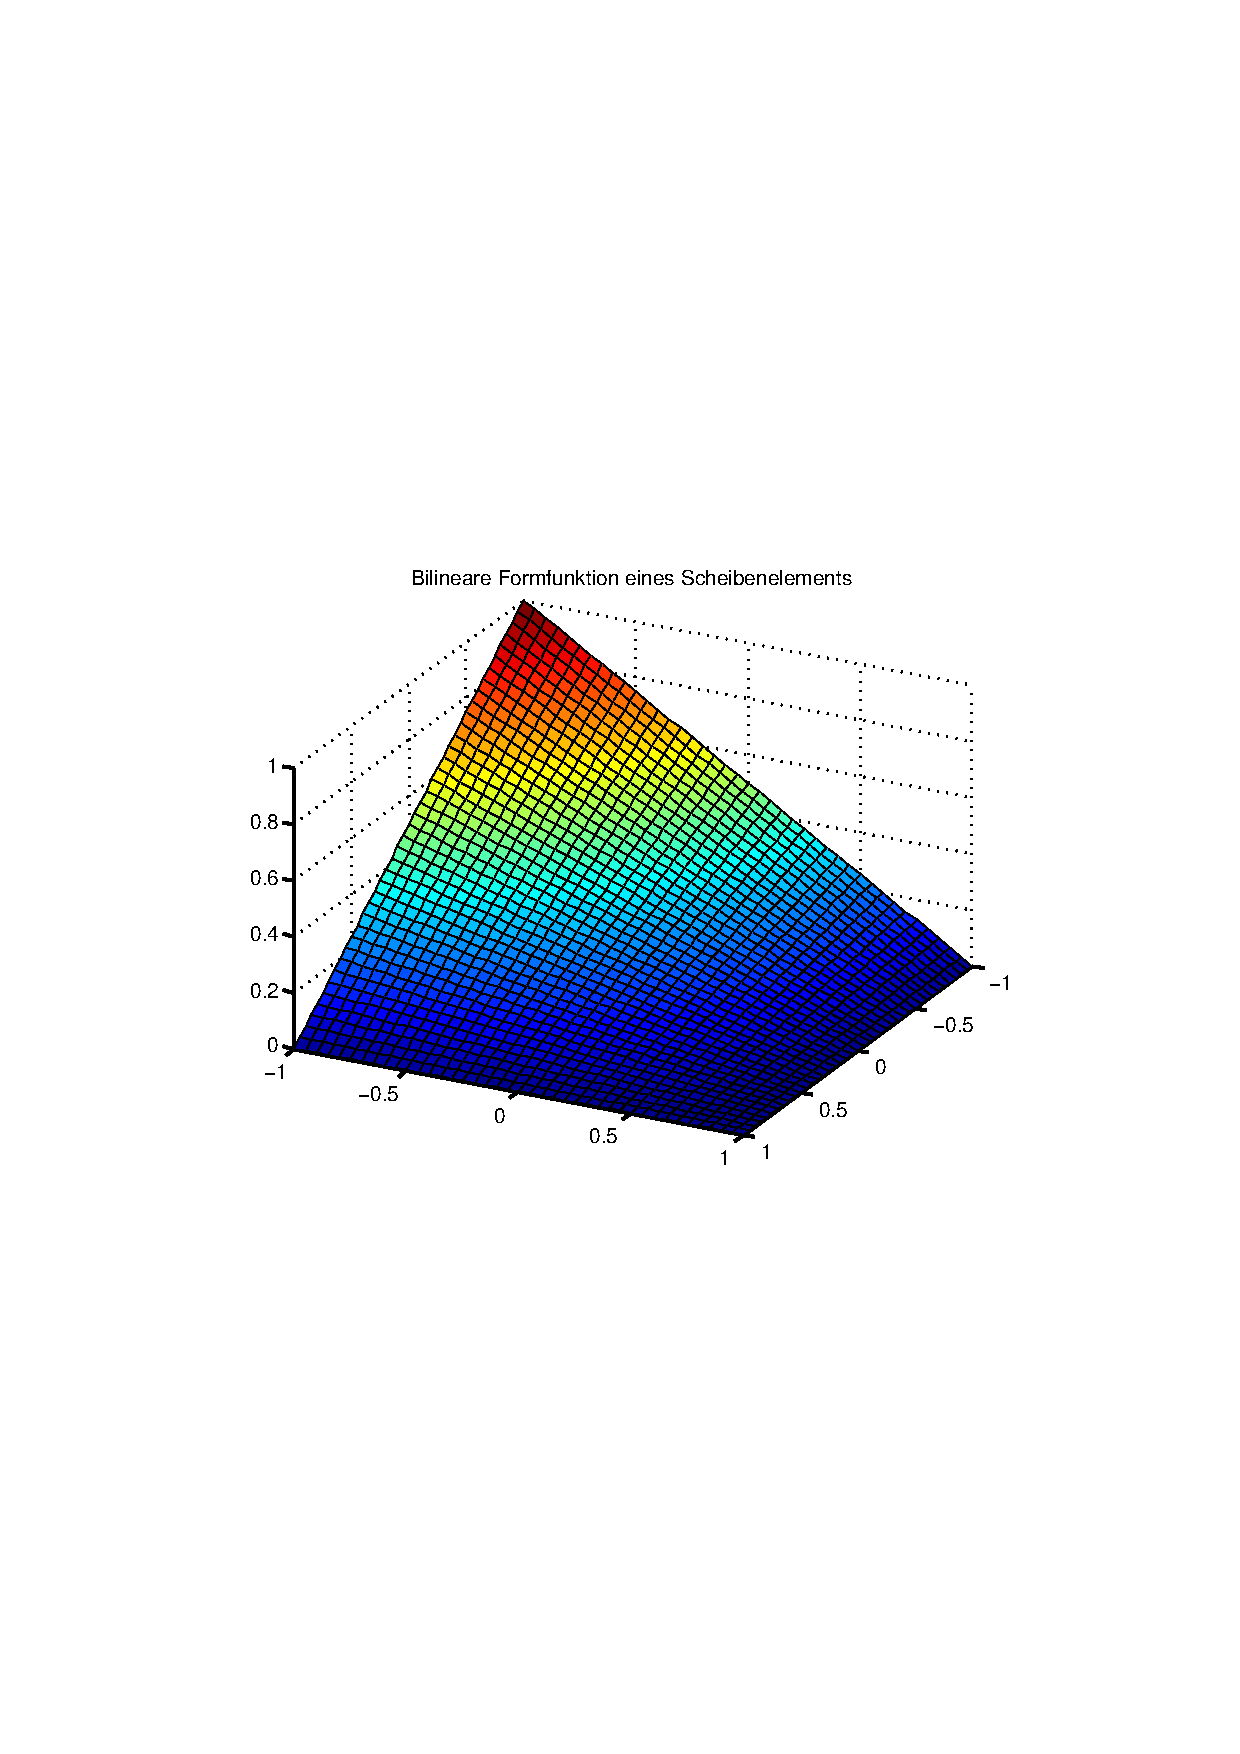
\includegraphics[width=0.4\textwidth]{bilder/140710_bilineare_Formfunktion.pdf}
	\caption{Beispielhafte Darstellung einer bilinearen Formfunktion f�r ein Scheibenelement}
	\label{fig:140710_bilineare_Formfunktion}
\end{figure}
Um den Unterschied zu einer "`Pixelgrafik"' zu sehen, einfach mal ganz weit in die Abbildung zoomen. Das Bild bleibt immer scharf!

\subsection{Tabellen einf�gen}
\label{sec:TabellenEinf�gen}

Tabellen werden unter Tabelle $\rightarrow$ einf�gen erstellt!

Beispiel:

\begin{table} [H]
\centering
\caption{Versuchsergebnisse zur Ermittlung der Federsteifigkeiten der elastischen Zwischenplatte Zwp BSP FF-B-1; Zulassungspr�fungen an der TU M�nchen}
\begin{tabular}{|c|c|c|c|} \hline  
\rowcolor[gray]{.9} 
 Pr�ftemperatur & stat. Steifigkeit $c_{stat}$ & dyn. Steifigkeit $c_{dyn}$ & Pr�ffrequenz \\\hline 
\rowcolor[gray]{.9} 
 $[�C]$                & $[kN/mm]$ & $[kN/mm]$ & $[Hz]$ \\\hline 
 50  & 33,6 & -    & -           \\\hline 
 50  & -    & 42,1 & 10        \\\hline
 23  & 33,0 & -    & -           \\\hline 
\end{tabular} 
\label{tab:Steifigkeiten_Zwp_TUM}
\end{table}


Beispiel "`Farbig"':

Nachfolgend ein Beispiel zum Erstellen von farbigen Tabellen:

\definecolor{LightCyan}{rgb}{0.88,1,1}           % Definieren der gew�nschten Farben
\definecolor{leichtesGelb}{rgb}{0.9,0.9,0}
\definecolor{maroon}{cmyk}{0,0.87,0.68,0.32}

\begin{table} [H]
\centering
\caption{Beispiel farbige Tabelle}
\begin{tabular}{|c|c|c|c|} \hline  
\rowcolor[gray]{.9} 
 Lastfallnr. & Bezeichnung des Modells & max. $w_{zz}$ (vertikal) & max. $v_{yy}$ (horizontal) \\\hline 
\rowcolor[gray]{.9} 
 $[-]$ & $[-]$ & $[mm]$ & $[mm]$ \\\hline 

\rowcolor{LightCyan}
\textcolor{red} 1 & {Stabwerk mit 5 Stp.}  & \textcolor{red} {1,86} & \textcolor{red} {0,00}    \\\hline 
\rowcolor{LightCyan}
1 & Volumen mit 5 Stp.  & 1,85 & 0,00     \\\hline 
\rowcolor{LightCyan}
\textcolor{red} 1 & {Stabwerk mit 6 Stp.}  & \textcolor{red} {1,87} & \textcolor{red} {0,00}   \\\hline 
\rowcolor{LightCyan}
1 & Volumen mit 6 Stp.  & 1,89 & 0,00   \\\hline 

\rowcolor{leichtesGelb!20}
\textcolor{red} 2 & {Stabwerk mit 5 Stp.}  & \textcolor{red} {1,86} & \textcolor{red} {0,34}    \\\hline 
\rowcolor{leichtesGelb!20}
2 & Volumen mit 5 Stp.  & 1,90 & 0,41     \\\hline
\rowcolor{leichtesGelb!20}
\textcolor{red} 2 & {Stabwerk mit 6 Stp.}  & \textcolor{red} {1,87} & \textcolor{red} {0,32}   \\\hline 
\rowcolor{leichtesGelb!20}
2 & Volumen mit 6 Stp.  & 1,91 & 0,36   \\\hline 

\textcolor{red} 3 & {Stabwerk mit 5 Stp.}  & \textcolor{red} {1,61} & \textcolor{red} {3,56}    \\\hline 
3 & Volumen mit 5 Stp.  & 1,64 & 3,25    \\\hline 
\textcolor{red} 3 & {Stabwerk mit 6 Stp.}  & \textcolor{red} {1,62} & \textcolor{red} {3,57}   \\\hline 
3 & Volumen mit 6 Stp.  & 1,65 & 3,31  \\\hline 
\end{tabular}

\label{tab:farbigeTabelle} 
\vspace{0.0cm}
\end{table} 



Die Tabellen werden automatisch in das Tabellenverzeichnis eingetragen!

\section{Sonstiges}
\label{sec:Sonstiges}

F�r weitere Informationen ist die "`LaTeX Kurzbeschreibung"' vom Leibniz Rechenzentrum sehr hilfreich: \href{https://www.lrz.de/services/software/textverarbeitung/tex/l2kurz.pdf} {Benutzerhandbuch - LaTeX} \\
Um Schnell etwas zu suchen, ist es zumeist am einfachsten das Zeichen oder das Problem zu "`googlen"'. Zur Erstellung von Arbeiten mit LaTeX gibt es unz�hlige Foren usw.

Viel Erfolg und Spa� beim Erstellen der Arbeit!














 
	